% 1977 年新疆卷（文科）第六题：拦水坝梯形横断面 ABCD（AD 为坝顶，BC 为坝底），
% AE、DF 为坝高的垂线（虚线），左侧水面示意短线，角 B=30°、角 C=45°，
% 坝顶上方标 2.5 尺寸线（按源卷第 4 页布局；比例约 1:2.2，非严格尺寸）
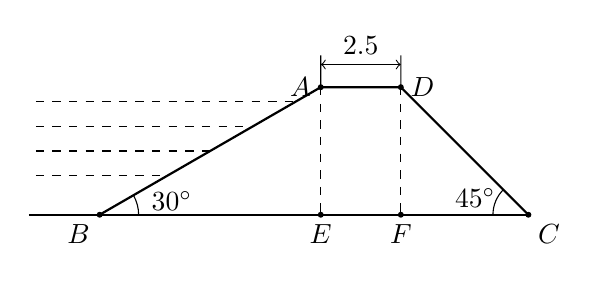
\begin{tikzpicture}[scale=0.9]
  \coordinate (B) at (0,0);
  \coordinate (E) at (3.12,0);
  \coordinate (F) at (4.25,0);
  \coordinate (C) at (6.05,0);
  \coordinate (A) at (3.12,1.8);
  \coordinate (D) at (4.25,1.8);
  \draw[thick] (-1.0,0)--(C);
  \draw[thick] (B)--(A)--(D)--(C);
  \draw[dashed] (A)--(E);
  \draw[dashed] (D)--(F);
  % 水面示意短线（迎水坡一侧）
  \draw[dashed] (-0.9,0.55)--(0.95,0.55);
  \draw[dashed] (-0.9,0.90)--(1.56,0.90);
  \draw[dashed] (-0.9,1.25)--(2.17,1.25);
  \draw[dashed] (-0.9,1.60)--(2.77,1.60);
  % 坝顶 2.5 尺寸标注
  \draw[thin] (A)--(3.12,2.25);
  \draw[thin] (D)--(4.25,2.25);
  \draw[<->] (3.12,2.12)--(4.25,2.12) node[midway,above] {$2.5$};
  % 角标注
  \draw (0.55,0) arc[start angle=0,end angle=30,radius=0.55];
  \node at (1.02,0.20) {$30^\circ$};
  \draw ([shift={(180:0.5)}]C) arc[start angle=180,end angle=135,radius=0.5];
  \node at (5.30,0.24) {$45^\circ$};
  \fill (A) circle (1.2pt) node[left] {$A$};
  \fill (D) circle (1.2pt) node[right] {$D$};
  \fill (B) circle (1.2pt) node[below left] {$B$};
  \fill (E) circle (1.2pt) node[below] {$E$};
  \fill (F) circle (1.2pt) node[below] {$F$};
  \fill (C) circle (1.2pt) node[below right] {$C$};
\end{tikzpicture}
